\documentclass[12pt]{article}

\usepackage{blindtext} % Package to generate dummy text throughout this template 

\usepackage[utf8]{inputenc}
\usepackage{amsmath, amssymb}
\usepackage{algorithm}
\usepackage[noend]{algpseudocode}
\linespread{1.25}
\usepackage[margin = 1in]{geometry}
\usepackage{microtype} % Slightly tweak font spacing for aesthetics
\usepackage[english]{babel} % Language hyphenation and typographical rules
\usepackage{tikz}
\usepackage{hyperref}
\usepackage{url}
\usepackage{graphicx}
\usepackage{float}
\usepackage{wrapfig}
\usepackage{multicol}
\usepackage{subcaption}
\hypersetup{
    colorlinks=true,
    linkcolor=red,      
    urlcolor=blue,
    bookmarks=true,
    citecolor=green!75!black
}

\setlength{\parindent}{2em}
%\setlength{\parskip}{1.5em}
\graphicspath{ {images/} }

\newcommand{\vect}[1]{\mathbf{#1}}  % vector
\newcommand{\matr}[1]{\mathbf{#1}}  % matrix
\newcommand{\tens}[1]{\mathbf{#1}}  % tensor
\newcommand{\mean}[1]{\overline{#1}}    % mean overline

\begin{document}
    \tableofcontents
    \listoftables
    \listoffigures
    \section{Introduction} \label{sec:Introduction}
    Optimizing predictive models on datasets that are obtained from citizen-science projects can be computationally expensive as these datasets grow in size with time. Consequently, models based on multiple-layered neural networks, Integer Programming and other optimization routines can prove increasingly difficult as the number of parameters increase, despite using the faster Central Processing Units (CPUs) in the market. Incidentally, it becomes difficult for citizen-science projects to scale if the organizers use CPUs to run optimization models. However, Graphical Processing Units (GPUs), which offer multiple cores to parallelize computation, can outperform CPUs in computing such predictive models if these models heavily rely on large-scale matrix multiplications. By using GPUs over CPUs to accelerate computation on a citizen-science project, the model could achieve better optimization in less time, enabling the project to scale.\\
    
    Part of the eBird project, which aims to ``maximize the utility and accessibility of the vast numbers of bird observations made each year by recreational and professional bird watchers'', Avicaching is a incentive-driven game trying to homogenize the spatial distribution of citizens' (agents') observations [cite website]. Since the dataset of agents' observations in eBird is geographically heterogeneous (concentrated in some places like cities and sparse in others), Avicaching homogenizes the observation set by rewarding agents who visit under-sampled locations \cite{Xue2016Avi1}. To accomplish this task of specifying rewards at different locations based on the historical records of observations, Avicaching would learn the change in agents' behavior when a certain sample of rewards were applied to the set of locations, and then distribute a newer set of rewards across the locations based on those learned parameters \cite{Xue2016Avi2}. This requirement naturally translates into a predictive optimization problem, which is implemented using multiple-layered neural networks and linear programming.

    \subsection{Computation Using GPUs} \label{sec:comp_using_GPUs}
    
    \section{Problem Formulation} \label{sec:Problem Formulation}
    Since NVIDIA General Purpose GPUs enable faster computation on matrices, accelerated through CUDA and cuDNN, both the Identification (Section \ref{sec:Identification Problem}) and the Pricing Problem (Section \ref{sec:Pricing Problem}) were formulated as 3-layered neural networks using the PyTorch library.
    
    \subsection{Identification Problem} \label{sec:Identification Problem}
    As discussed in Section \ref{sec:Introduction}, the model should learn parameters that caused the change in agents' behavior when a certain set of rewards was applied to locations in the experiment region. Specifically, given datasets $\vect{y_t}$ and $\vect{x_t}$ of agents' visit densities with and without the rewards $\vect{r_t}$, we want to find weights $\matr{w_1}$ and $\matr{w_2}$ that caused the change from $\vect{x_t}$ to $\vect{y_t}$, factoring in possible influence from environmental factors $\matr{f}$ and distances between locations $\matr{D}$. Although the original model proposed to learn a single set of weights $\matr{w}$ \cite{Xue2016Avi2}, this proposed model considers two sets of weights $\matr{w_1}$ and $\matr{w_2}$ as it may theoretically result into higher accuracy and lower loss. Mathematically, the model can be formulated as:
    \begin{equation} \label{eq:iden_problem}
    \begin{aligned}
    & \underset{\matr{w_1}, \matr{w_2}}{\text{minimize}}
    & & Z_I(\matr{w_1}, \matr{w_2}) = \sum_{t} (\omega(\vect{y_t} - \matr{P}(\matr{f}, \vect{r_t}; \matr{w_1}, \matr{w_2})\vect{x_t}))^{2}
    \end{aligned}
    \end{equation}
    where $\omega$ is a set of weights at time $t$ capturing penalties relative to the importance of homogenizing at different locations and elements $p_{u, v}$ of $\matr{P}$ are given as:
    \begin{equation} \label{eq:puv_equation}
    p_{u, v} = \frac{\exp(\matr{w_2} \cdot \text{reLU} (\matr{w_1} \cdot [d_{u, v}, \vect{f_{u}}, r_{u}]))}{\sum_{u'} \exp(\matr{w_2} \cdot \text{reLU} (\matr{w_1} \cdot [d_{u', v}, \vect{f_{u'}}, r_{u'}]))} = \frac{\exp(\Gamma_{u, v})}{\sum_{u'}\exp(\Gamma_{u', v})} = \text{softmax}(\Gamma_{u, v})
    \end{equation}
    In the expression for $p_{u,v}$ (Equation \ref{eq:puv_equation}), softmax$(\cdot)$ is the function: softmax$(z_i) = \frac{\exp(z_i)}{\sum_{i}\exp(z_i)}$ and the reLU$(\cdot)$ function is a ``rectified Linear Unit'' defined as: reLU$(z) = \text{max}(0, z)$.\\
    To optimize the loss value $Z_I(\matr{w_1}, \matr{w_2})$ (Equation \ref{eq:iden_problem}), the neural network learns the set of weights through multiple iterations of backpropagating the loss using gradient descent. Furthermore, the program processes the dataset before feeding to the network to avoid unnecessary sub-iterations and promote batch operations on matrices. 
    
    \subsubsection{Structure of Input Dataset for Identifying Weights} \label{sec:Structure of Input Dataset for Identifying Weights}
    \begin{figure}[H]
        \begin{subfigure}{.64\textwidth}
            \centering
            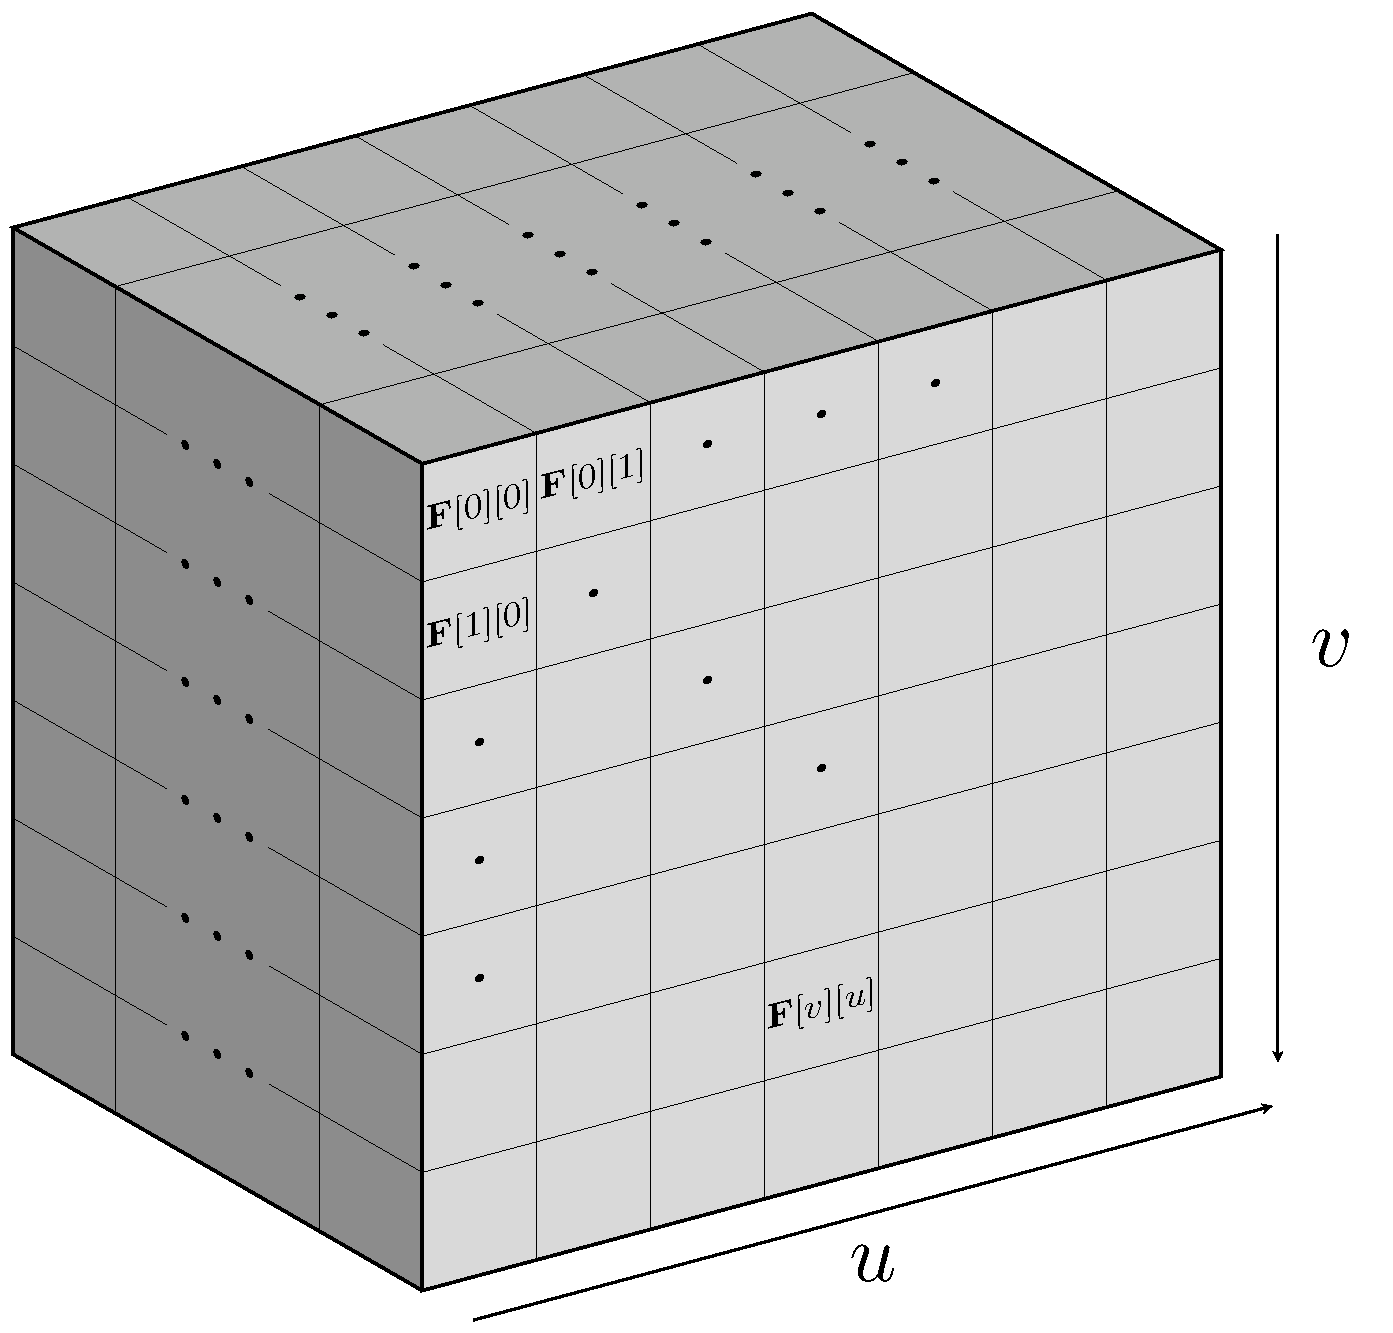
\includegraphics[width=\linewidth]{weights_input_dataset}
            \caption{A Tensor representing the Input Dataset $\matr{F}$}
            \label{fig:A Tensor representing the complete Input Dataset}
        \end{subfigure}
        \begin{subfigure}{.35\textwidth}
            \centering
            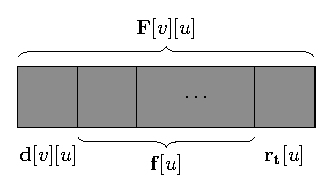
\includegraphics[width=\linewidth]{zoomup_Fuv}
            \caption{Contents of $\matr{F}[v][u]$}
            \label{fig:Zoomed-in contents of Fvu}
        \end{subfigure}
        \caption{Visual representation of the Input Dataset}
        \label{fig:Visual representation of the Input Dataset}
    \end{figure}
    Since preprocessing the dataset impacts the efficiency of the network, the input dataset, comprising of distance between locations $\matr{D}$, environmental features $\vect{f}$ and given rewards $\vect{r_t}$ (all normalized) are combined in a specific manner. Since GPUs are efficient in operating on matrices and tensors, the input dataset is built into a tensor (Figure \ref{fig:A Tensor representing the complete Input Dataset}) such that batch operations could be performed on slices $\matr{F}[v]$. Another advantage of building the dataset as a tensor comes with the PyTorch library, which provides convenient handling and transfer of tensors residing on CPUs and GPUs. Algorithm \ref{alg:Constructing the Input Dataset} describes the steps to construct this dataset.
    \begin{algorithm}
        \caption{Constructing the Input Dataset} \label{alg:Constructing the Input Dataset}
        \begin{algorithmic}[1]
            \Function{Build-Dataset}{$\matr{D}, \matr{f}, \matr{r_t}$}
            \State $\matr{D} \gets \Call{Normalize}{\matr{D}}$\Comment{$\matr{D}[u][v]$ is the distance between locations $u$ and $v$}
            \State $\vect{f} \gets \Call{Normalize}{\mathbf{f}, axis = 0}$\Comment{$\mathbf{f}[u]$ is a vector of env. features at location $u$}
            \State $\vect{r_t} \gets \Call{Normalize}{\vect{r_t}, axis = 0}$\Comment{$\vect{r_t}[u]$ is the reward at location $u$}
            \For{$v = 1, 2, \dots, J$}
                \For{$u = 1, 2, \dots, J$}
                    \State $\tens{F}[v][u] \gets [\matr{D}[v][u], \vect{f}[u], \vect{r_t}[u]]$ \Comment{As depicted in Figure \ref{fig:Zoomed-in contents of Fvu}}
                 \EndFor
            \EndFor
            \State \Return $\matr{F}$
            \EndFunction
        \end{algorithmic}
    \end{algorithm}
       
    \subsubsection{Minimizing Loss for the Identification Problem} \label{sec:Minimizing Loss for the Identification Problem}
    As shown in Figure \ref{fig:Neural network designed for the Identification Problem}, the neural network is made of 3 fully connected layers - the input layer, the hidden layer with rectified Linear Units (reLU), and the output layer generating the results using the softmax$(\cdot)$ function. The network can also be visualized as a collection of 1-dimensional layers (Figure \ref{fig:Side view of the network}), with the softmax$(\cdot)$ calculated on the collection's output.
    \begin{figure}[H]
        \begin{subfigure}{.64\textwidth}
        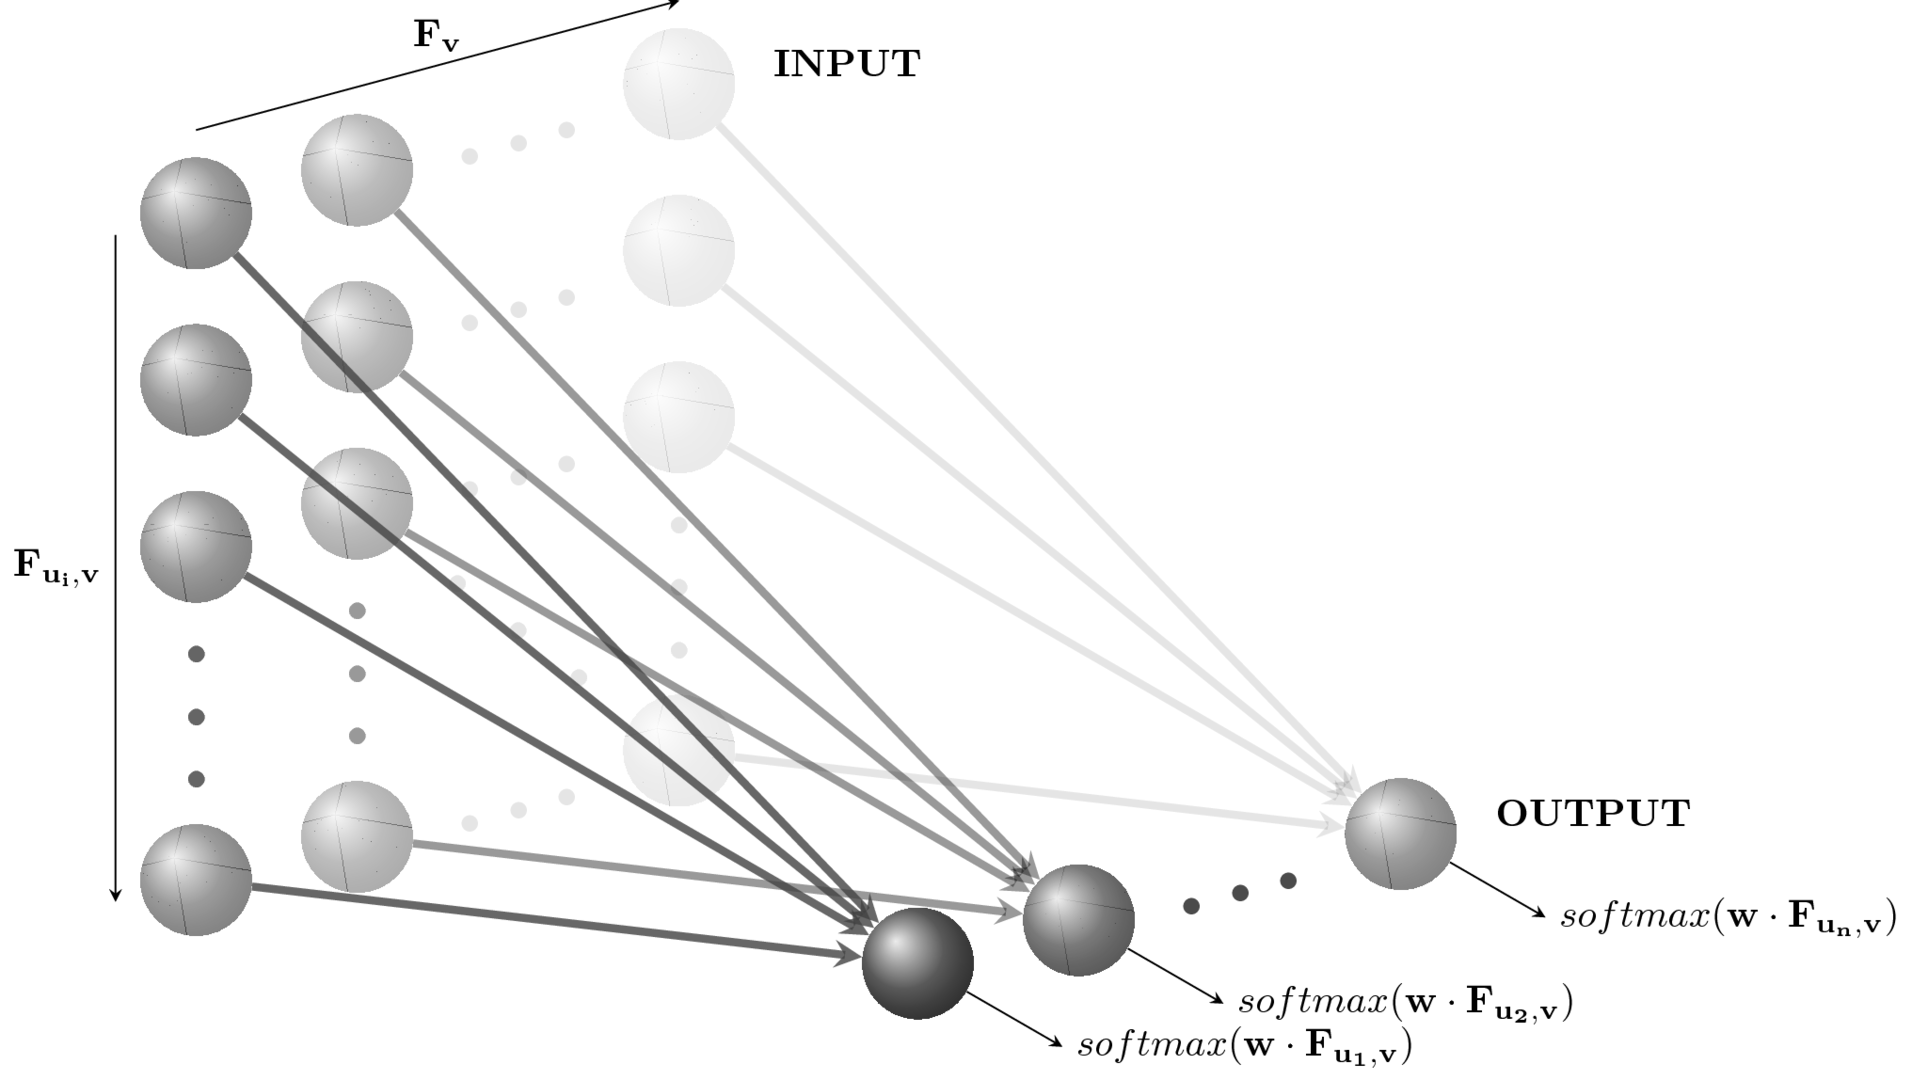
\includegraphics[width=\textwidth]{weights_net}
        \caption{3-dimensional view of the network slice, taking in $\matr{F}[v]$}
        \label{fig:3-dimensional view of the network slice, taking in Fv}
        \end{subfigure}
        \begin{subfigure}{.35\textwidth}
            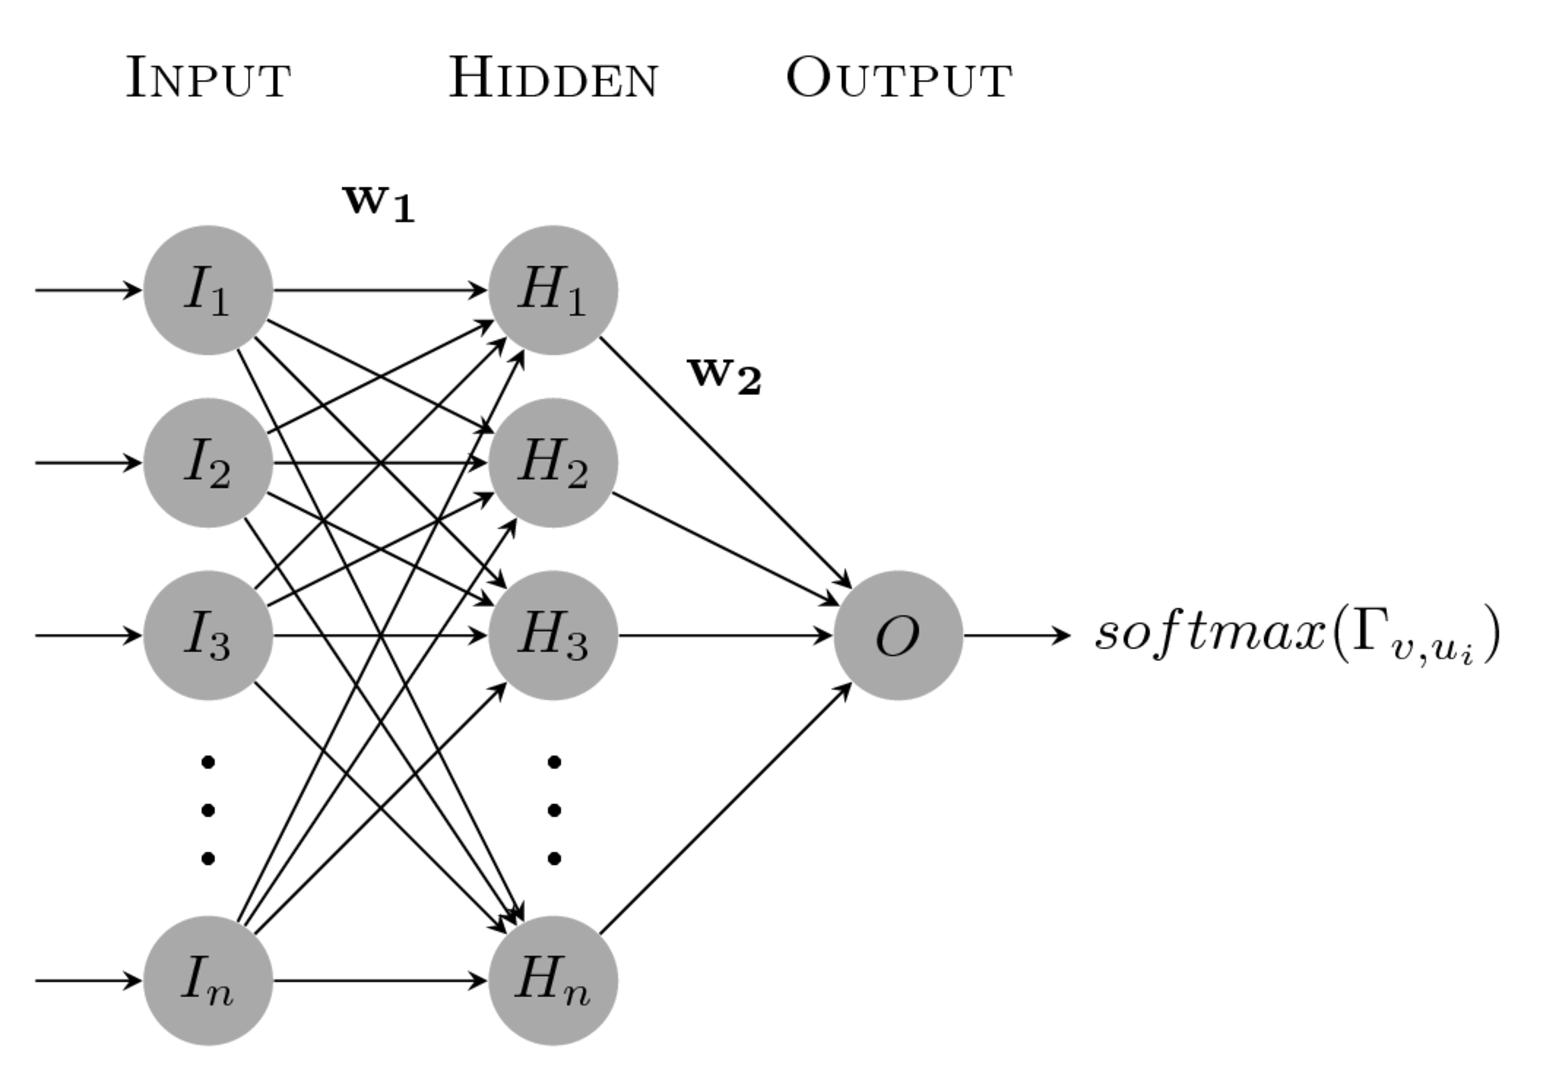
\includegraphics[width=\textwidth]{weights_net_side}
            \caption{Side view of the network}
            \label{fig:Side view of the network}
        \end{subfigure}
        \caption{Neural network designed for the Identification Problem}
        \label{fig:Neural network designed for the Identification Problem}
    \end{figure}
    It is important to clarify that the network in Figure \ref{fig:3-dimensional view of the network slice, taking in Fv}, which takes in $\matr{F}[v]$ as shown, is a slice of the original network, which takes in the complete tensor $\matr{F}$ and computes the complete result $\matr{P}^{T}$  per iteration of $t$. In other words, the input and the hidden layers are 3-dimensional, and the output layer is 2-dimensional. Since it is difficult to visualize the complete network on paper, slices of the network are depicted in Figure \ref{fig:3-dimensional view of the network slice, taking in Fv}. Algorithm \ref{alg:Algorithm for the Identification Problem per iteration} details the steps for learning the parameters $\matr{w_1}$ and $\matr{w_2}$ based on Equations \ref{eq:iden_problem} \& \ref{eq:puv_equation}.
    \begin{algorithm}
        \caption{Algorithm for the Identification Problem per iteration} \label{alg:Algorithm for the Identification Problem per iteration}
        \begin{algorithmic}[1]
            \Require $\matr{w_1}, \matr{w_2}, T$
            \Function{Identify-Weights}{$\matr{x}, \matr{y}, \matr{r}, \matr{D}, \matr{f}, \omega$}
            \For{$t = 1, 2, \dots, T$}
                \State $\matr{F} \gets \Call{Build-Dataset}{\matr{D}, \matr{f}, \matr{r}[t]}$\Comment{Defined in Algorithm \ref{alg:Constructing the Input Dataset}}
                \State $\matr{\Lambda} \gets \text{reLU}(\Call{Batch-Multiply}{\matr{F}, \matr{w_1}})$\Comment{\textbf{Phase 1: Feed Forward}}
                \State $\matr{\Gamma} \gets \text{softmax}(\Call{Batch-Multiply}{\matr{\Lambda}, \matr{w_2}})$
                \State $\matr{P} \gets \matr{\Gamma}^T$
                \State $loss \gets loss + (\omega(\matr{y}[t] - \matr{P} \cdot \matr{x}[t]))^2$
            \EndFor
            \State $\Call{Gradient-Descent}{loss, \matr{w_1}, \matr{w_2}}$\Comment{\textbf{Phase 2: Backpropagate}}
            \State $\matr{w_1}, \matr{w_2} \gets \Call{Update-Using-Gradients}{\matr{w_1}, \matr{w_2}}$
            \State \Return $loss$
            \EndFunction
        \end{algorithmic}
    \end{algorithm}

    \subsection{Pricing Problem} \label{sec:Pricing Problem}
    After learning the set of weights $\matr{w_1}$ and $\matr{w_2}$ highlighting the change in agents' behavior to collect observations, the Pricing Problem aims to redistribute rewards to the all locations such that the predicted behavior of agents influenced by the new set of rewards is homogeneous. Thus, given a budget of rewards $\mathcal{R}$, this optimization problem can be expressed as:
    \begin{equation} \label{eq:pricing_problem}
    \begin{aligned}
    & \underset{\vect{r}}{\text{minimize}}
    & & Z_P(\vect{r}) = \frac{1}{n}\lVert \vect{y} - \mean{\vect{y}} \rVert\\
    & \text{subject to}
    & & \vect{y} = \matr{P}(\matr{f}, \vect{r}; \matr{w_1}, \matr{w_2}) \, \vect{x}\\
    &&& \sum_{i} r_i \leq \mathcal{R}\\
    &&& r_i \geq 0
    \end{aligned}
    \end{equation}
    where elements of $\matr{P}$ are defined as in Equation \ref{eq:puv_equation}. 
    To allocate the rewards $\vect{r}$ optimally, the calculations for the pricing problem are akin to that for the Identification Problem (Section \ref{sec:Identification Problem}). However, since only 1 set of rewards need to be optimized, we use an altered 2-layer network instead of the 3-layer network used to identify the weights. While Equation \ref{eq:pricing_problem} looks like a typical Linear Programming problem, only a part of the formulation uses Linear Programming to constrain the rewards. The more computationally expensive part (calculation for $\matr{P}$ on a CPU) is modeled as a 2-layer network that minimizes the loss function $Z_P(\vect{r})$ using gradient descent. Although this use of a neural network may seem similar to that of the Identification Problem, there are major changes in the structure of the network used here. These alterations for the Pricing Problem and differences from the Identification Problem are discussed further in the following sections.
    
    \subsubsection{Input Dataset for Finding Rewards}
    
    Since it is the set of rewards $\vect{r}$ that need to be optimized, they must serve as the ``weights'' of the network (note that ``weights'' refer to the edges of this network and not to the set of calculated weights $\matr{w_1}$ and $\matr{w_2}$). Therefore, the rewards $\vect{r}$ are no longer fed into the network but are its characteristic. Instead, the calculated weights $\matr{w_1}$ are fed into the network, and are ``weighted'' by the rewards.\\
    
    The observation density datasets, $\matr{x}$ and $\matr{y}$, are also aggregated for all agents such that they give information in terms of locations $u$ only. This is also why rewards $\vect{r}$ does not depend on $t$ - we want a generalized set of rewards for all time $t$ per location $u$. Therefore, the algorithm for constructing $\matr{F}$ (Section \ref{sec:Structure of Input Dataset for Identifying Weights}) is same as Algorithm \ref{alg:Constructing the Input Dataset} but with a change - $\vect{r_t}$ replaced by $\vect{r}$.
    
    \subsubsection{Optimizing \& Constraining Rewards}
    The algorithm for finding $\matr{P}$ is very similar to Phase 1 of Algorithm \ref{alg:Algorithm for the Identification Problem per iteration} but without any iterations of $t$, as $\vect{x}$ is a vector rather than a matrix. Also, since the program would predict $\vect{y}$, it does not need labels $\vect{y}$ as a dataset.\\
    
    \begin{algorithm}
        \caption{Solving the Pricing Problem} \label{alg:Solving the Pricing Problem}
        \begin{algorithmic}[1]
            \Function{Optimize-Rewards}{$\vect{x}, \matr{w_1}, \matr{w_2}, \matr{D}, \matr{f}$}
            \Require $\vect{r}, \mathcal{R}$
            \State $\matr{F} \gets \Call{Build-Dataset}{\matr{D}, \matr{f}, \vect{r}}$\Comment{Defined in Algorithm \ref{alg:Constructing the Input Dataset}}
            \State $\matr{\Lambda} \gets \text{reLU}(\Call{Batch-Multiply}{\matr{F}, \matr{w_1}})$\Comment{\textbf{Phase 1: Solve for $\matr{P}$ and $loss$}}
            \State $\matr{\Gamma} \gets \text{softmax}(\Call{Batch-Multiply}{\matr{\Lambda}, \matr{w_2}})$
            \State $\matr{P} \gets \matr{\Gamma}^T$
            \State $\vect{y} \gets \matr{P} \cdot \vect{x}$
            \State $loss \gets \lVert \vect{y} - \mean{\vect{y}} \rVert / J$\Comment{$J$ is the number of locations}
            \State $\Call{Gradient-Descent}{loss, \vect{r}}$\Comment{\textbf{Phase 2: Backpropagate}}
            \State $\vect{r} \gets \Call{Update-Using-Gradients}{\vect{r}}$
            \State $\vect{r} \gets \Call{LP}{\vect{r}, \mathcal{R}}$\Comment{LP($\cdot$) explained below}
            \State \Return $loss$
            \EndFunction
        \end{algorithmic}
    \end{algorithm}
    After updating the rewards, the program constrains them using LP($\cdot$) such that $\sum_{i}r_i \leq \mathcal{R}$ and $r_i \geq 0$. To do so, the LP($\cdot$) finds another set of rewards $\vect{r'}$ such that the absolute difference between new and old rewards ($\sum_{i}|r'_i - r_i|$) is minimum. The mathematical formulation is given in Equation \ref{eq:lp_math_constrain_rewards}, which was implemented using SciPy's Optimize Module []. Since the module supports a standard format\footnote{minimize [$\vect{c}^T \cdot \vect{x}$]; subject to [$\matr{A} \cdot \vect{x} \leq \vect{b}, \, x_i \geq 0$]} for doing linear programming, Equation \ref{eq:lp_code_constrain_rewards} (after rearranging constraints and building $\matr{A}, \vect{b}$ and $\vect{c}$) is used, which is mathematically equivalent to Equation \ref{eq:lp_math_constrain_rewards}.
    \begin{multicols}{2}
        \begin{equation} \label{eq:lp_math_constrain_rewards}
        \begin{aligned}
            & \underset{\vect{r'}}{\text{minimize}}
            & & \sum_{i}|r'_i - r_i|\\ \\
            & \text{subject to}
            & & \sum_{i}r'_i \leq \mathcal{R}\\
            &&& r_i \geq 0
        \end{aligned}
        \end{equation}\break
        \begin{equation} \label{eq:lp_code_constrain_rewards}
        \begin{aligned}
            & \underset{\vect{r'}, \vect{u}}{\text{minimize}}
            & & \sum_{i} u_i\\
            & \text{subject to}
            & & r'_i - r_i \leq u_i\\
            &&& r_i - r'_i \leq u_i\\
            &&& \sum_{i} r'_i \leq \mathcal{R}\\
            &&& r'_i, u_i \geq 0
        \end{aligned}
        \end{equation}
    \end{multicols}
    \section{Experiments}
    
    \section{Results}
    \section{Conclusion}
    
    \blindtext
    \bibliographystyle{ieeetr}
    \bibliography{avicaching}
\end{document}